\documentclass[10pt,a4paper]{article}
%-------------------------------------------
%---Packages--------------------------------
%-------------------------------------------
\usepackage[utf8]{inputenc}
%\usepackage[T1]{fontenc}
%\usepackage{txfonts}
\usepackage{amsmath}
\usepackage{amsthm}
\usepackage{amsfonts}
\usepackage{array}
\usepackage{amssymb}
\usepackage{blindtext}
\usepackage{caption}
\usepackage{color}
\usepackage{csquotes}	    %
\usepackage{enumitem}	    %pour mieux bosser avec les listes. ajoute option label
\usepackage[yyyymmdd]{datetime}        %pour définir date custom
\usepackage{etaremune}    
\usepackage{environ}
\usepackage{fancybox}
\usepackage{fancyhdr} 	    % Custom headers and footers
\usepackage{fancyref}
%\usepackage{float}
\usepackage{floatrow}       %float and floatrow can't be together...
\usepackage{gensymb}
\usepackage{graphicx}
\usepackage[colorlinks=true, linkcolor=purple, citecolor=cyan]{hyperref}
\usepackage{footnotebackref}
\usepackage{lipsum}
\usepackage{mathtools}
\usepackage{multicol}	    %gérer plusieurs colonnes
\usepackage{setspace}
\usepackage{subcaption}
\usepackage{todonotes}	    %Bonne gestion des TODOs
%TODO commenté pour tester l'utilité... à voir% \usepackage[tc]{titlepic}      %Permet de mettre une image en page de garde
\usepackage{tikz}	    % Pour outil de dessin puissant 
\usepackage{ulem}	    %underline sur plusieurs lignes (avec \uline{})
\usepackage{vmargin} 	    %gestion des marges, avec dans l'ordre : gauche, haut, droit, bas, en-tête, entre en-tête et texte, bas de page, hauteur entre bas de page et texte 
\usepackage{wrapfig}
\usepackage{xcolor}
\usepackage{xparse}                    %Pour utiliser NewDocumentCommand et des arguments 'mmooo'
%\usepackage{fullpage} 	    %supprime toutes les marges allouées aux notes, aussi en haut et en bas

%\ExplSyntaxOn
\pagestyle{fancyplain}	    %Makes all pages in the document conform to the custom headers and footers

%-------------------------------------------
%---Document Commands-----------------------
%---------------------------{----------------
\NewDocumentCommand{\framecolorbox}{oommm}
 {% #1 = width (optional)
  % #2 = inner alignment (optional)
  % #3 = frame color
  % #4 = background color
  % #5 = text
  \IfValueTF{#1}%
   {\IfValueTF{#2}%
    {\fcolorbox{#3}{#4}{\makebox[#1][#2]{#5}}}%
    {\fcolorbox{#3}{#4}{\makebox[#1]{#5}}}%
   }%
   {\fcolorbox{#3}{#4}{#5}}%
 }%
%------------------------------------------------
%------------------ENGLISH----------------------
%----------------------------------------------

\NewDocumentCommand{\epflTitle}{mO{Olivier Cloux}O{\today}O{Notes de Cours en}D<>{../../Common}}%Arguments : Matière, Auteur, Date, Titre du doc
{
\begin{titlepage}
    \vspace*{\fill}
    \begin{center}
        \normalfont \normalsize 
        \textsc{Ecole Polytechnique Fédérale de Lausanne} \\ [25pt] % Your university, school and/or department name(s)
        \textsc{#4} %Titre du doc
        \\ [0.4 pt]
        \horrule{0.5pt} \\[0.4cm] % Thin top horizontal rule
        \huge #1 \\ % Matière
        \horrule{2pt} \\[0.5cm] % Thick bottom horizontal rule
        \includegraphics[width=8cm]{#5/EPFL_logo}
        ~\\[0.5 cm]
        \small\textsc{#2}\\[0.4cm]
        \small\textsc{#3}\\
        ~\\
        ~\\
        \includegraphics[scale=0.5]{#5/creativeCommons}
    \end{center}
    \vspace*{\fill}
\end{titlepage}
}


%-------------------------------------------
%-------------MATH NEW COMMANDS-------------
%-------------------------------------------
\newcommand{\somme}[2]{\ensuremath{\sum\limits_{#2}^{#1}}}
\newcommand{\produit}[2]{\ensuremath{\prod\limits_{#2}^{#1}}}
\newcommand{\limite}{\lim\limits_}
\newcommand{\llimite}[3]{\limite{\substack{#1 \\ #2}}\left(#3\right)}	%limites à deux condiitons
\newcommand{\et}{\mbox{ et }}
\newcommand{\deriv}[1]{\ensuremath{\, \mathrm d #1}}	%sigle dx, dt,dy... des dérivées/intégrales
%\newcommand{\fx}{\ensuremath{f'(\textbf{x}_0 + h}}
\newcommand{\ninf}{\ensuremath{n \to \infty}}	       %pour les limites : n tend vers l'infini
\newcommand{\xinf}{\ensuremath{x \to \infty}}	       %pour les limites : x tend vers l'infini
\newcommand{\infint}{\ensuremath{\int_{-\infty}^{\infty}}}
\newcommand{\xo}{\ensuremath{x \to 0}}									%x to 0
\newcommand{\no}{\ensuremath{n \to 0}}									%n zéro
\newcommand{\xx}{\ensuremath{x \to x}}									%x to x
\newcommand{\Xo}{\ensuremath{x_0}}										%x zéro
\newcommand{\X}{\ensuremath{\mathbf{X}} }
\newcommand{\A}{\ensuremath{\mathbf{A}} }
\newcommand{\R}{\ensuremath{\mathbb{R}} }								%ensemble de R
\newcommand{\rn}{\ensuremath{\mathbb{R}^n} } 							%ensemble de R de taille n
\newcommand{\Rm}{\ensuremath{\mathbb{R}^m} }  							%ensemble de R de taille m
\newcommand{\C}{\ensuremath{\mathbb{C}} } 		
\newcommand{\N}{\ensuremath{\mathbb{N}} }
\newcommand{\Z}{\ensuremath{\mathbb{Z}} }
\newcommand{\Q}{\ensuremath{\mathbb{Q}} }
\newcommand{\rtor}{\ensuremath{\R \to \R} }
\newcommand{\pour}{\mbox{ pour }}
\newcommand{\coss}[1]{\ensuremath{\cos\(#1\)}}						%cosinus avec des parenthèses de bonne taille (genre frac)
\newcommand{\sinn}[1]{\ensuremath{\sin\(#1\)}}					%sinus avec des parentèses de bonne taille (genre frac)
\newcommand{\txtfrac}[2]{\ensuremath{\frac{\text{#1}}{\text{#2}}}}		%Fractions composées de texte
\newcommand{\evalfrac}[3]{\ensuremath{\left.\frac{#1}{#2}\right|_{#3}}}
\renewcommand{\(}{\left(}												%Parenthèse gauche de taille adaptive
\renewcommand{\)}{\right)}
\newcommand{\longeq}{=\joinrel=}												%Parenthèse droite de taille adaptive


%-------------------------------------------------------
%------------------MISC NEW COMMANDS--------------------
%-------------------------------------------------------
\newcommand{\degre}{\ensuremath{^\circ}}
%\newdateformat{\eudate}{\THEYEAR-\twodigit{\THEMONTH}-\twodigit{\THEDAY}}



%-------------------------------------------------------
%------------------TEXT NEW COMMANDS--------------------
%-------------------------------------------------------
\newcommand{\ts}{\textsuperscript}
\newcommand{\evid}[1]{\textbf{\uline{#1}}}        %mise en évidence (gras + souligné)



%\newcommand{\Exemple}{\underline{Exemple}}
\newcommand{\Theoreme}{\underline{Théorème}}
\newcommand{\Remarque}{\underline{Remarque}}
\newcommand{\Definition}{\underline{Définition} }
\newcommand{\skinf}{\sum^{\infty}_{k=0}}
\newcommand{\combi}[2]{\ensuremath{\begin{pmatrix} #1 \\ #2 \end{pmatrix}}}	%combinaison parmi 1 de 2
\newcommand{\intx}[3]{\ensuremath{\int_{#1}^{#2} #3 \deriv{x}}}				%intégrale dx
\newcommand{\intt}[3]{\ensuremath{\int_{#1}^{#2} #3 \deriv{t}}}				%intégrale dy
\newcommand{\misenforme}{\begin{center} Mis en forme jusqu'ici\\ \line(1,0){400}\\ normalement juste, mais à améliorer depuis ici\end{center}}	%raccourci pour mise en forme
\newcommand*\circled[1]{\tikz[baseline=(char.base)]{
            \node[shape=circle,draw,inner sep=1pt] (char) {#1};}}			%pour entourer un chiffre
\newcommand{\horrule}[1]{\rule{\linewidth}{#1}} 				% Create horizontal rule command with 1 argument of height

\theoremstyle{definition}
\newtheorem{exemp}{Exemple}
\newtheorem{examp}{Example}


%-------------------------------------------
%---Environments----------------------------
%-------------------------------------------
\NewEnviron{boite}[1][0.9]{%
	\begin{center}
		\framecolorbox{red}{white}{%
			\begin{minipage}{#1\textwidth}
 	 			\BODY
			\end{minipage}
		}
	\end{center}
}
\NewEnviron{blackbox}[1][0.9]{%
	\begin{center}
		\framecolorbox{black}{white}{%
			\begin{minipage}{#1\textwidth}
 	 			\BODY
			\end{minipage}
		}
	\end{center}
}
\NewEnviron{exemple}[1][0.8]{%
    \begin{center}
        \framecolorbox{white}{gray!20}{%
            \begin{minipage}{#1\textwidth}
                \begin{exemp}
                    \BODY
                \end{exemp}
            \end{minipage}
        }
    \end{center}
}
\NewEnviron{suiteExemple}[1][0.8]{%
    \begin{center}
        \framecolorbox{white}{gray!20}{%
            \begin{minipage}{#1\textwidth}
                \BODY
            \end{minipage}
        }
    \end{center}
}
\NewEnviron{colExemple}[1][0.8]{%
    \begin{center}
        \framecolorbox{white}{gray!20}{%
            \begin{minipage}{#1\columnwidth}
                \begin{exemp}
                    \BODY
                \end{exemp}
            \end{minipage}
        }
    \end{center}
}
\NewEnviron{example}[1][0.8]{%
    \begin{center}
        \framecolorbox{white}{gray!20}{%
            \begin{minipage}{#1\textwidth}
                \begin{examp}
                    \BODY
                \end{examp}
            \end{minipage}
	}
    \end{center}
}
\NewEnviron{systeq}[1][l]{
			\begin{center}
				$\left\{\begin{array}{#1}
					\BODY
				\end{array}\right.$
			\end{center}
 }





%-------------------------------------------
%---General settings-----------------------
%-------------------------------------------
\renewcommand{\headrulewidth}{1pt}										%ligne au haut de chaque page
\renewcommand{\footrulewidth}{1pt}										%ligne au pied de chaque page
\setstretch{1.6}
\author{Olivier Cloux}
\usepackage{tikz}
\setlength{\leftmargin}{0pt}
\setlength{\rightmargin}{0pt}
\title{Série 2}
\date{}
\begin{document}
\maketitle
\part*{236079}
\evid{Problème 2.1}\\
\begin{enumerate}
	\item Pour les codes A,B,D, l'alphabet du code est $\{0,1\}$ (la source sera \enquote{traduite} dans dans cet alphabet), alors que pour l'alphabet du code C est $\{0,1,2\}$. Pour tous les codes, l'alphabet de la source est $\{a,b,c,d,e,f\}$  (chaque caractère de la source vient de cet alphabet). Finalement, chaque code a un dictionnaire spécifique :
	\begin{itemize}
		\item[Code A] $\{1010, 01, 001, 0001, 11, 011\}$
		\item[Code B] $\{0, 11, 101, 100, 001, 010\}$
		\item[Code C] $\{1,12,122,10,102,100\}$
		\item[Code D] $\{10, 011, 111, 00, 0101, 1100\}$
	\end{itemize}
	\newpage
	\item 
		\begin{itemize}
			\item Code A :
		\end{itemize}	 
\end{enumerate}
	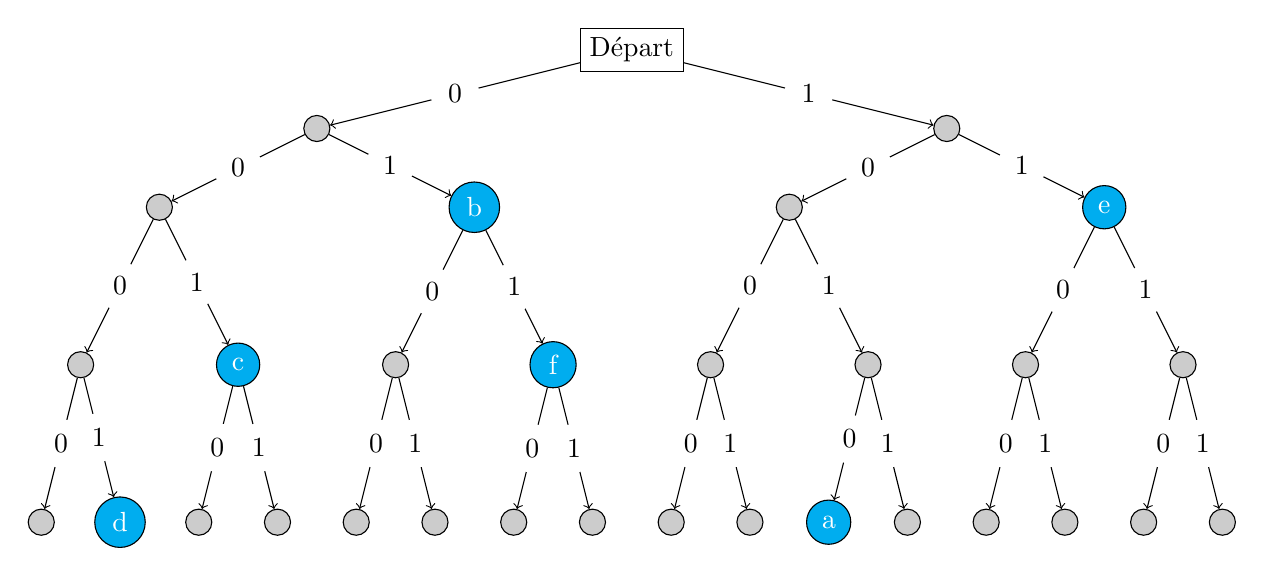
\begin{tikzpicture}[scale=0.5]
		\tikzstyle{etiquette}=[midway, circle ,fill=white]
		\node[draw] (D) at (0,0){Départ};	
		\node[draw, circle, fill=black!20] (1) at (8,-2){};
		\node[draw, circle, fill=black!20] (0) at (-8,-2){};
		\node[draw, circle, fill=cyan, text=white] (11) at (12,-4){e};
		\node[draw, circle, fill=black!20] (10) at (4,-4){};
		\node[draw, circle, fill=cyan, text=white] (01) at (-4,-4){b};
		\node[draw, circle, fill=black!20] (00) at (-12,-4){};
		\node[draw, circle, fill=black!20] (111) at (14,-8){};
		\node[draw, circle, fill=black!20] (110) at (10,-8){};
		\node[draw, circle, fill=black!20] (101) at (6,-8){};
		\node[draw, circle, fill=black!20] (100) at (2,-8){};
		\node[draw, circle, fill=cyan, text=white] (011) at (-2,-8){f};
		\node[draw, circle, fill=black!20] (010) at (-6,-8){};
		\node[draw, circle, fill=cyan, text=white] (001) at (-10,-8){c};
		\node[draw, circle, fill=black!20] (000) at (-14,-8){};
		\node[draw, circle, fill=black!20] (1111) at (15,-12){};
		\node[draw, circle, fill=black!20] (1110) at (13,-12){};
		\node[draw, circle, fill=black!20] (1101) at (11,-12){};
		\node[draw, circle, fill=black!20] (1100) at (9,-12){};
		\node[draw, circle, fill=black!20] (1011) at (7,-12){};
		\node[draw, circle, fill=cyan, text=white] (1010) at (5,-12){a};
		\node[draw, circle, fill=black!20] (1001) at (3,-12){};
		\node[draw, circle, fill=black!20] (1000) at (1,-12){};
		\node[draw, circle, fill=black!20] (0111) at (-1,-12){};
		\node[draw, circle, fill=black!20] (0110) at (-3,-12){};
		\node[draw, circle, fill=black!20] (0101) at (-5,-12){};
		\node[draw, circle, fill=black!20] (0100) at (-7,-12){};
		\node[draw, circle, fill=black!20] (0011) at (-9,-12){};
		\node[draw, circle, fill=black!20] (0010) at (-11,-12){};
		\node[draw, circle, fill=cyan, text=white] (0001) at (-13,-12){d};
		\node[draw, circle, fill=black!20] (0000) at (-15,-12){};

		\draw[->] (D) -- (0)node[etiquette]{0};
		\draw[->] (D) -- (1)node[etiquette]{1};
		\draw[->] (0) -- (00)node[etiquette]{0};
		\draw[->] (0) -- (01)node[etiquette]{1};
		\draw[->] (1) -- (10)node[etiquette]{0};
		\draw[->] (1) -- (11)node[etiquette]{1};
		\draw[->] (00) -- (000)node[etiquette]{0};
		\draw[->] (00) -- (001)node[etiquette]{1};
		\draw[->] (01) -- (010)node[etiquette]{0};
		\draw[->] (01) -- (011)node[etiquette]{1};
		\draw[->] (10) -- (100)node[etiquette]{0};
		\draw[->] (10) -- (101)node[etiquette]{1};
		\draw[->] (11) -- (110)node[etiquette]{0};
		\draw[->] (11) -- (111)node[etiquette]{1};
		\draw[->] (000) -- (0000)node[etiquette]{0};
		\draw[->] (000) -- (0001)node[etiquette]{1};
		\draw[->] (001) -- (0010)node[etiquette]{0};
		\draw[->] (001) -- (0011)node[etiquette]{1};
		\draw[->] (010) -- (0100)node[etiquette]{0};
		\draw[->] (010) -- (0101)node[etiquette]{1};
		\draw[->] (011) -- (0110)node[etiquette]{0};
		\draw[->] (011) -- (0111)node[etiquette]{1};
		\draw[->] (100) -- (1000)node[etiquette]{0};
		\draw[->] (100) -- (1001)node[etiquette]{1};
		\draw[->] (101) -- (1010)node[etiquette]{0};
		\draw[->] (101) -- (1011)node[etiquette]{1};
		\draw[->] (110) -- (1100)node[etiquette]{0};
		\draw[->] (110) -- (1101)node[etiquette]{1};
		\draw[->] (111) -- (1110)node[etiquette]{0};
		\draw[->] (111) -- (1111)node[etiquette]{1};
	\end{tikzpicture}\\
	\\
		\begin{itemize}
	 	\item Code B
	\end{itemize}
\begin{center}
		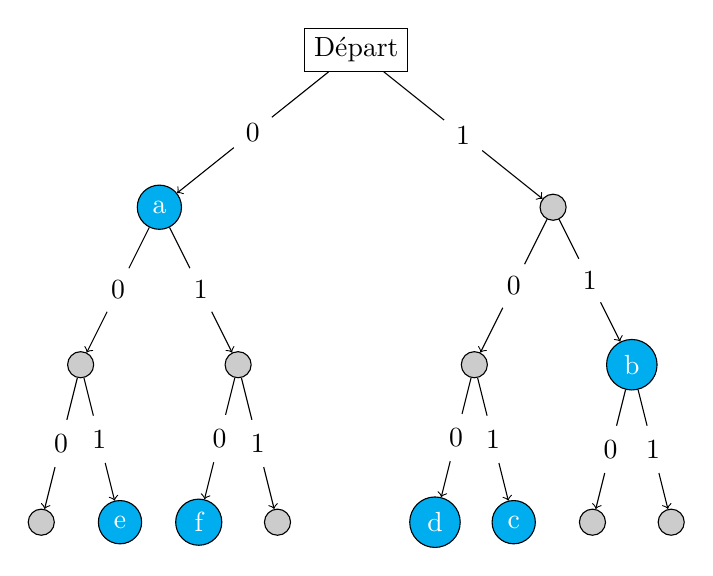
\begin{tikzpicture}[scale=1]
		\tikzstyle{etiquette}=[midway, circle ,fill=white]
		\node[draw] (D) at (0,0){Départ};	
		\node[draw, circle, fill=black!20] (1) at (2.5,-2){};
		\node[draw, circle, fill=cyan, text=white] (0) at (-2.5,-2){a};
		\node[draw, circle, fill=cyan, text=white] (11) at (3.5,-4){b};
		\node[draw, circle, fill=black!20] (10) at (1.5,-4){};
		\node[draw, circle, fill=black!20] (01) at (-1.5,-4){};
		\node[draw, circle, fill=black!20] (00) at (-3.5,-4){};
		\node[draw, circle, fill=black!20] (111) at (4,-6){};
		\node[draw, circle, fill=black!20] (110) at (3,-6){};
		\node[draw, circle, fill=cyan, text=white] (101) at (2,-6){c};
		\node[draw, circle, fill=cyan, text=white] (100) at (1,-6){d};
		\node[draw, circle, fill=black!20] (011) at (-1,-6){};
		\node[draw, circle, fill=cyan, text=white] (010) at (-2,-6){f};
		\node[draw, circle, fill=cyan, text=white] (001) at (-3,-6){e};
		\node[draw, circle, fill=black!20] (000) at (-4,-6){};

		\draw[->] (D) -- (0)node[etiquette]{0};
		\draw[->] (D) -- (1)node[etiquette]{1};
		\draw[->] (0) -- (00)node[etiquette]{0};
		\draw[->] (0) -- (01)node[etiquette]{1};
		\draw[->] (1) -- (10)node[etiquette]{0};
		\draw[->] (1) -- (11)node[etiquette]{1};
		\draw[->] (00) -- (000)node[etiquette]{0};
		\draw[->] (00) -- (001)node[etiquette]{1};
		\draw[->] (01) -- (010)node[etiquette]{0};
		\draw[->] (01) -- (011)node[etiquette]{1};
		\draw[->] (10) -- (100)node[etiquette]{0};
		\draw[->] (10) -- (101)node[etiquette]{1};
		\draw[->] (11) -- (110)node[etiquette]{0};
		\draw[->] (11) -- (111)node[etiquette]{1};
	\end{tikzpicture}\\
\end{center}
\newpage
	\begin{itemize}
		\item Code C:
		\end{itemize}
		\begin{center}
			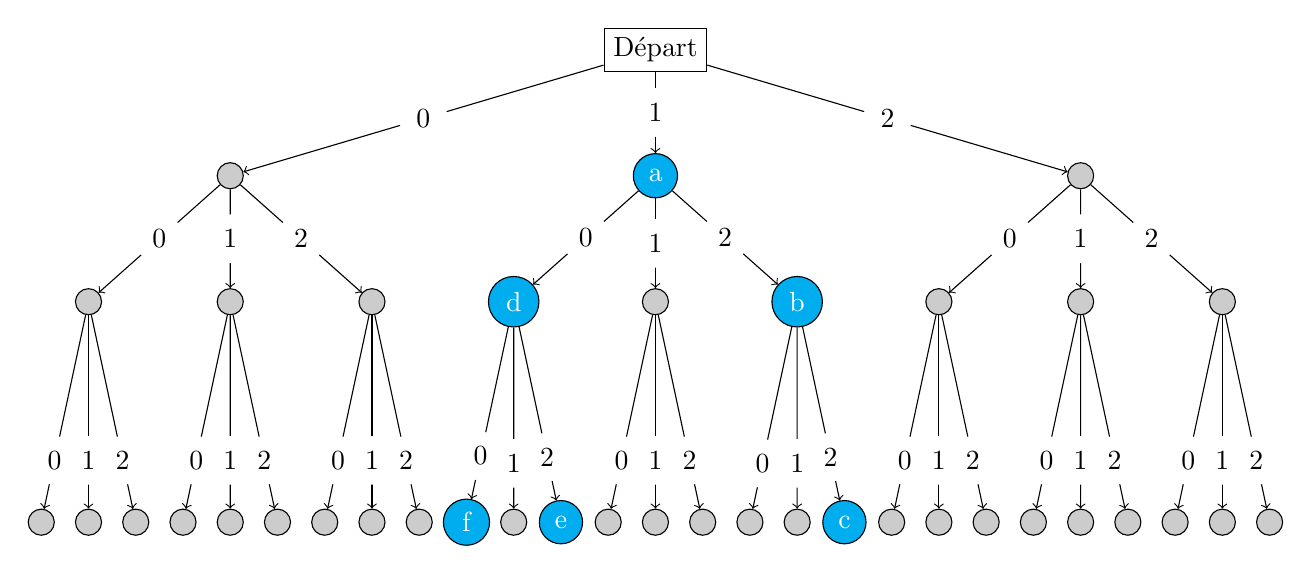
\begin{tikzpicture}[scale=0.4]
			%#######################################################
			%##################Stlyes###############################
			%#######################################################
				\tikzstyle{etiquette}=[near end, circle ,fill=white]
				\tikzstyle{etiquette_mid}=[midway, circle, fill=white]
				
			%#######################################################
			%##################Points###############################
			%#######################################################
				\node[draw] (D) at (0,0){Départ};
				\node[draw, circle, fill=black!20] (000) at (-19.5, -15){};				
				\node[draw, circle, fill=black!20] (001) at (-18, -15){};
				\node[draw, circle, fill=black!20] (002) at (-16.5, -15){};
				\node[draw, circle, fill=black!20] (010) at (-15, -15){};
				\node[draw, circle, fill=black!20] (011) at (-13.5, -15){};
				\node[draw, circle, fill=black!20] (012) at (-12, -15){};
				\node[draw, circle, fill=black!20] (020) at (-10.5, -15){};
				\node[draw, circle, fill=black!20] (021) at (-9, -15){};
				\node[draw, circle, fill=black!20] (022) at (-7.5, -15){};
				\node[draw, circle, fill=cyan, text=white] (100) at (-6, -15){f};
				\node[draw, circle, fill=black!20] (101) at (-4.5, -15){};
				\node[draw, circle, fill=cyan, text=white] (102) at (-3, -15){e};
				\node[draw, circle, fill=black!20] (110) at (-1.5, -15){};
				\node[draw, circle, fill=black!20] (111) at (0,-15){};
				\node[draw, circle, fill=black!20] (112) at (1.5,-15){};
				\node[draw, circle, fill=black!20] (120) at (3,-15){};
				\node[draw, circle, fill=black!20] (121) at (4.5,-15){};
				\node[draw, circle, fill=cyan, text=white] (122) at (6,-15){c};
				\node[draw, circle, fill=black!20] (200) at (7.5,-15){};
				\node[draw, circle, fill=black!20] (201) at (9,-15){};
				\node[draw, circle, fill=black!20] (202) at (10.5,-15){};
				\node[draw, circle, fill=black!20] (210) at (12,-15){};
				\node[draw, circle, fill=black!20] (211) at (13.5,-15){};
				\node[draw, circle, fill=black!20] (212) at (15,-15){};
				\node[draw, circle, fill=black!20] (220) at (16.5,-15){};
				\node[draw, circle, fill=black!20] (221) at (18,-15){};
				\node[draw, circle, fill=black!20] (222) at (19.5,-15){};
				
				\node[draw, circle, fill=black!20] (00) at (-18, -8){};
				\node[draw, circle, fill=black!20] (01) at (-13.5, -8){};
				\node[draw, circle, fill=black!20] (02) at (-9, -8){};
				\node[draw, circle, fill=cyan, text=white] (10) at (-4.5, -8){d};
				\node[draw, circle, fill=black!20] (11) at (0, -8){};
				\node[draw, circle, fill=cyan, text=white] (12) at (4.5, -8){b};
				\node[draw, circle, fill=black!20] (20) at (9, -8){};
				\node[draw, circle, fill=black!20] (21) at (13.5, -8){};
				\node[draw, circle, fill=black!20] (22) at (18, -8){};
				
				\node[draw, circle, fill=black!20] (0) at (-13.5, -4){};
				\node[draw, circle, fill=cyan, text=white] (1) at (0,-4){a};
				\node[draw, circle, fill=black!20] (2) at (13.5,-4){};
				
			%#######################################################
			%##################Traits###############################
			%#######################################################
				\draw[->] (D) -- (0)node[etiquette_mid]{0};
				\draw[->] (D) -- (1)node[etiquette_mid]{1};
				\draw[->] (D) -- (2)node[etiquette_mid]{2};
				
				\draw[->] (0) -- (00)node[etiquette_mid]{0};
				\draw[->] (0) -- (01)node[etiquette_mid]{1};
				\draw[->] (0) -- (02)node[etiquette_mid]{2};
				\draw[->] (1) -- (10)node[etiquette_mid]{0};
				\draw[->] (1) -- (11)node[etiquette_mid]{1};
				\draw[->] (1) -- (12)node[etiquette_mid]{2};
				\draw[->] (2) -- (20)node[etiquette_mid]{0};
				\draw[->] (2) -- (21)node[etiquette_mid]{1};
				\draw[->] (2) -- (22)node[etiquette_mid]{2};
				\draw[->] (00) -- (000)node[etiquette]{0};
				\draw[->] (00) -- (001)node[etiquette]{1};
				\draw[->] (00) -- (002)node[etiquette]{2};
				\draw[->] (01) -- (010)node[etiquette]{0};
				\draw[->] (01) -- (011)node[etiquette]{1};
				\draw[->] (01) -- (012)node[etiquette]{2};
				\draw[->] (02) -- (020)node[etiquette]{0};
				\draw[->] (02) -- (021)node[etiquette]{1};
				\draw[->] (02) -- (022)node[etiquette]{2};
				\draw[->] (10) -- (100)node[etiquette]{0};
				\draw[->] (10) -- (101)node[etiquette]{1};
				\draw[->] (10) -- (102)node[etiquette]{2};
				\draw[->] (11) -- (110)node[etiquette]{0};
				\draw[->] (11) -- (111)node[etiquette]{1};
				\draw[->] (11) -- (112)node[etiquette]{2};
				\draw[->] (12) -- (120)node[etiquette]{0};
				\draw[->] (12) -- (121)node[etiquette]{1};
				\draw[->] (12) -- (122)node[etiquette]{2};
				\draw[->] (20) -- (200)node[etiquette]{0};
				\draw[->] (20) -- (201)node[etiquette]{1};
				\draw[->] (20) -- (202)node[etiquette]{2};
				\draw[->] (21) -- (210)node[etiquette]{0};
				\draw[->] (21) -- (211)node[etiquette]{1};
				\draw[->] (21) -- (212)node[etiquette]{2};
				\draw[->] (22) -- (220)node[etiquette]{0};
				\draw[->] (22) -- (221)node[etiquette]{1};
				\draw[->] (22) -- (222)node[etiquette]{2};
				
				
			\end{tikzpicture}
		\end{center}
		
		\begin{itemize}
	
		\item Code D:
	\end{itemize}
\begin{center}
		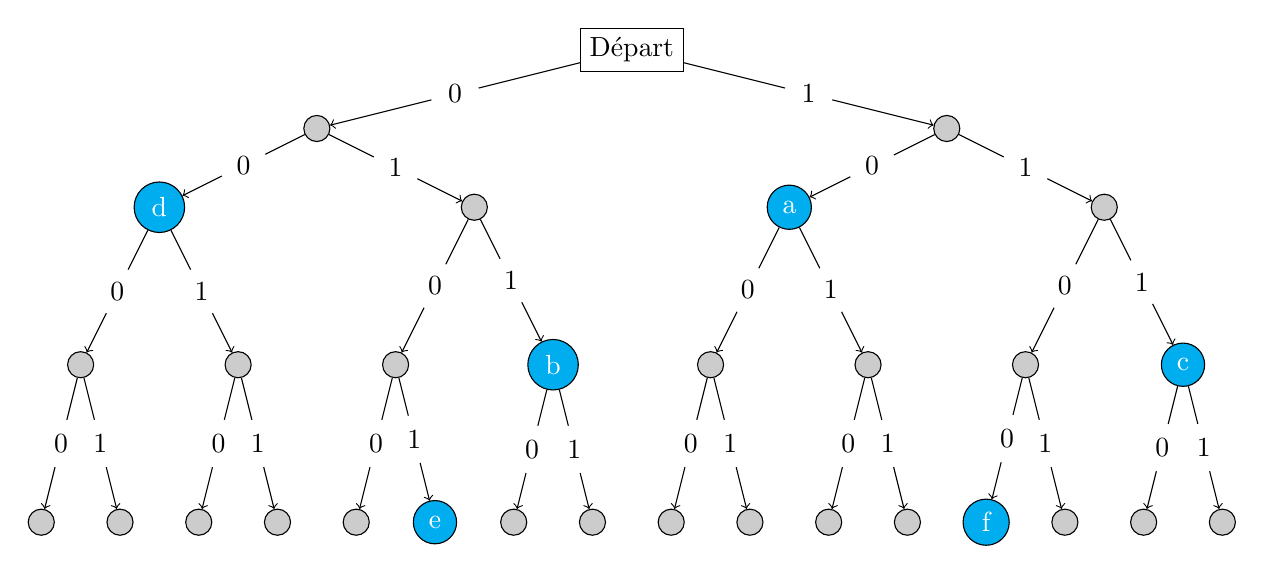
\begin{tikzpicture}[scale=0.5]
		\tikzstyle{etiquette}=[midway, circle ,fill=white]
		\node[draw] (D) at (0,0){Départ};	
		\node[draw, circle, fill=black!20] (1) at (8,-2){};
		\node[draw, circle, fill=black!20] (0) at (-8,-2){};
		\node[draw, circle, fill=black!20] (11) at (12,-4){};
		\node[draw, circle, fill=cyan, text=white] (10) at (4,-4){a};
		\node[draw, circle, fill=black!20] (01) at (-4,-4){};
		\node[draw, circle, fill=cyan, text=white] (00) at (-12,-4){d};
		\node[draw, circle, fill=cyan, text=white] (111) at (14,-8){c};
		\node[draw, circle, fill=black!20] (110) at (10,-8){};
		\node[draw, circle, fill=black!20] (101) at (6,-8){};
		\node[draw, circle, fill=black!20] (100) at (2,-8){};
		\node[draw, circle, fill=cyan, text=white] (011) at (-2,-8){b};
		\node[draw, circle, fill=black!20] (010) at (-6,-8){};
		\node[draw, circle, fill=black!20] (001) at (-10,-8){};
		\node[draw, circle, fill=black!20] (000) at (-14,-8){};
		\node[draw, circle, fill=black!20] (1111) at (15,-12){};
		\node[draw, circle, fill=black!20] (1110) at (13,-12){};
		\node[draw, circle, fill=black!20] (1101) at (11,-12){};
		\node[draw, circle, fill=cyan, text=white] (1100) at (9,-12){f};
		\node[draw, circle, fill=black!20] (1011) at (7,-12){};
		\node[draw, circle, fill=black!20] (1010) at (5,-12){};
		\node[draw, circle, fill=black!20] (1001) at (3,-12){};
		\node[draw, circle, fill=black!20] (1000) at (1,-12){};
		\node[draw, circle, fill=black!20] (0111) at (-1,-12){};
		\node[draw, circle, fill=black!20] (0110) at (-3,-12){};
		\node[draw, circle, fill=cyan, text=white] (0101) at (-5,-12){e};
		\node[draw, circle, fill=black!20] (0100) at (-7,-12){};
		\node[draw, circle, fill=black!20] (0011) at (-9,-12){};
		\node[draw, circle, fill=black!20] (0010) at (-11,-12){};
		\node[draw, circle, fill=black!20] (0001) at (-13,-12){};
		\node[draw, circle, fill=black!20] (0000) at (-15,-12){};

		\draw[->] (D) -- (0)node[etiquette]{0};
		\draw[->] (D) -- (1)node[etiquette]{1};
		\draw[->] (0) -- (00)node[etiquette]{0};
		\draw[->] (0) -- (01)node[etiquette]{1};
		\draw[->] (1) -- (10)node[etiquette]{0};
		\draw[->] (1) -- (11)node[etiquette]{1};
		\draw[->] (00) -- (000)node[etiquette]{0};
		\draw[->] (00) -- (001)node[etiquette]{1};
		\draw[->] (01) -- (010)node[etiquette]{0};
		\draw[->] (01) -- (011)node[etiquette]{1};
		\draw[->] (10) -- (100)node[etiquette]{0};
		\draw[->] (10) -- (101)node[etiquette]{1};
		\draw[->] (11) -- (110)node[etiquette]{0};
		\draw[->] (11) -- (111)node[etiquette]{1};
		\draw[->] (000) -- (0000)node[etiquette]{0};
		\draw[->] (000) -- (0001)node[etiquette]{1};
		\draw[->] (001) -- (0010)node[etiquette]{0};
		\draw[->] (001) -- (0011)node[etiquette]{1};
		\draw[->] (010) -- (0100)node[etiquette]{0};
		\draw[->] (010) -- (0101)node[etiquette]{1};
		\draw[->] (011) -- (0110)node[etiquette]{0};
		\draw[->] (011) -- (0111)node[etiquette]{1};
		\draw[->] (100) -- (1000)node[etiquette]{0};
		\draw[->] (100) -- (1001)node[etiquette]{1};
		\draw[->] (101) -- (1010)node[etiquette]{0};
		\draw[->] (101) -- (1011)node[etiquette]{1};
		\draw[->] (110) -- (1100)node[etiquette]{0};
		\draw[->] (110) -- (1101)node[etiquette]{1};
		\draw[->] (111) -- (1110)node[etiquette]{0};
		\draw[->] (111) -- (1111)node[etiquette]{1};
	\end{tikzpicture}\\
\end{center}
%\addtolength{\leftmargin}{40pt}
%\addtolength{\rightmargin}{40pt}
\begin{enumerate}[resume]
	\item 
	\begin{enumerate}
		\item Code A : $2^{-4}+2^{-2}+2^{-3}+2^{-4}+2^{-2}+2^{-3} = \frac{7}{8} \leq 1\\
		 \to$ Le code A respecte l'inégalité de Kraft.
		\item Code B : $2^{-1} + 2^{-2}+2^{-3}+2^{-3} + 2^{-3}+2^{-3} = \frac{5}{4} = 1.25 > 1 \\
		\to $ Le code B ne respecte \underline{pas} l'inégalité de Kraft.
		\item Code C :$3^{-1} + 3^{-2} + 3^{-3} + 3^{-2} + 3^{-3} + 3^{-3} = \frac{2}{3} = 0,\overline{6} \leq 1\\
		 \to$ Le code C respecte l'inégalité de Kraft.
		\item Code D :$2^{-2} + 2^{-3}+2^{-3}+2^{-2}+2^{-4}+2^{-4} = \frac{7}{8} \leq 1\\
		 \to$ Le code D respecte l'inégalité de Kraft.
	\end{enumerate}
\end{enumerate}
\paragraph{
Rappelons ici quelques implications générales, relatives à tous les codes que nous étudions ici:\\
sans préfixe $\iff$ instantané $\to$ à décodage unique\\
code à décodage unique $\to$ inégalité de Kraft respectée\\
Évidemment, si leurs contraposées sont exactes, leurs réciproques elles sont de manière générale fausses.}
\begin{enumerate}[resume]
	\item La première partie du théorème de Kraft, grossièrement, dit que si le code est à décodage unique, alors il satisfait l'inégalité de Kraft. Par contraposée, le fait que l'inégalité ne soit pas respectée implique que le code n'est pas à décodage unique. Ainsi, le code B n'est pas à décodage unique.
	\item Un code est à décodage unique si on ne peut jamais \enquote{mal interpréter} une suite valide. De plus, nous savons qu'un code à décodage instantané est à décodage unique également, raison pour laquelle nous pouvons affirmer que le code D est à décodage unique (preuve dans la question suivante).\\
	 Pour le code B, la séquence $ad = 0100 = fa$, donc il n'est pas à décodage unique.\\
	 Pour le A, la séquence $bab = 01101001 = fbc$, donc le code n'est pas à décodage unique.\\
	 En revanche, le code C est lui à décodage unique car les \enquote{1} sont uniquement au début de tous les mots ; pour déchiffrer un code il n'y a donc qu'à repérer les séquences délimitées par les \enquote{1}.
	\item Un code est à décodage instantané si et seulement s'il est sans préfixe ; c'est à dire qu'aucun mot du dictionnaire n'est le début d'un autre (par exemple le code \enquote{0} est préfixe de \enquote{0101}). Nous voyons donc bien que les codes A,B,C sont avec préfixes (donc pas à décodage instantané), alors que le code D est à décodage instantané (car sans préfixe).
	\item Arbre de décodage du code D
\end{enumerate}
\begin{center}
		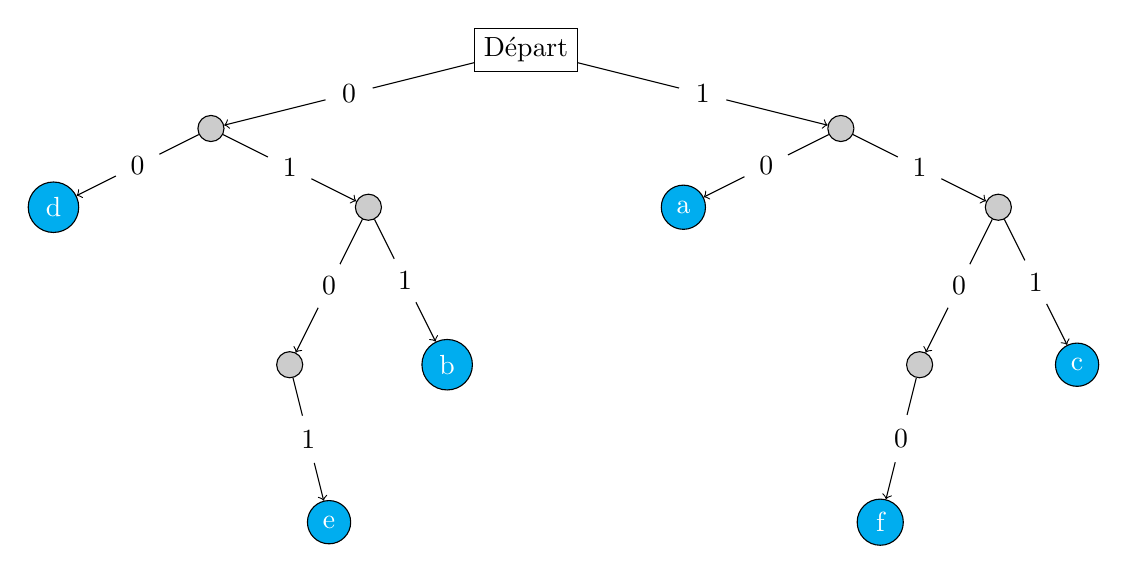
\begin{tikzpicture}[scale=0.5]
		\tikzstyle{etiquette}=[midway, circle ,fill=white]
		\node[draw] (D) at (0,0){Départ};	
		\node[draw, circle, fill=black!20] (1) at (8,-2){};
		\node[draw, circle, fill=black!20] (0) at (-8,-2){};
		\node[draw, circle, fill=black!20] (11) at (12,-4){};
		\node[draw, circle, fill=cyan, text=white] (10) at (4,-4){a};
		\node[draw, circle, fill=black!20] (01) at (-4,-4){};
		\node[draw, circle, fill=cyan, text=white] (00) at (-12,-4){d};
		\node[draw, circle, fill=cyan, text=white] (111) at (14,-8){c};
		\node[draw, circle, fill=black!20] (110) at (10,-8){};
%		\node[draw, circle, fill=black!20] (101) at (6,-8){};
%		\node[draw, circle, fill=black!20] (100) at (2,-8){};
		\node[draw, circle, fill=cyan, text=white] (011) at (-2,-8){b};
		\node[draw, circle, fill=black!20] (010) at (-6,-8){};
%		\node[draw, circle, fill=black!20] (001) at (-10,-8){};
%		\node[draw, circle, fill=black!20] (000) at (-14,-8){};
%		\node[draw, circle, fill=black!20] (1111) at (15,-12){};
%		\node[draw, circle, fill=black!20] (1110) at (13,-12){};
%		\node[draw, circle, fill=black!20] (1101) at (11,-12){};
		\node[draw, circle, fill=cyan, text=white] (1100) at (9,-12){f};
%		\node[draw, circle, fill=black!20] (1011) at (7,-12){};
%		\node[draw, circle, fill=black!20] (1010) at (5,-12){};
%		\node[draw, circle, fill=black!20] (1001) at (3,-12){};
%		\node[draw, circle, fill=black!20] (1000) at (1,-12){};
%		\node[draw, circle, fill=black!20] (0111) at (-1,-12){};
%		\node[draw, circle, fill=black!20] (0110) at (-3,-12){};
		\node[draw, circle, fill=cyan, text=white] (0101) at (-5,-12){e};
%		\node[draw, circle, fill=black!20] (0100) at (-7,-12){};
%		\node[draw, circle, fill=black!20] (0011) at (-9,-12){};
%		\node[draw, circle, fill=black!20] (0010) at (-11,-12){};
%		\node[draw, circle, fill=black!20] (0001) at (-13,-12){};
%		\node[draw, circle, fill=black!20] (0000) at (-15,-12){};

		\draw[->] (D) -- (0)node[etiquette]{0};
		\draw[->] (D) -- (1)node[etiquette]{1};
		\draw[->] (0) -- (00)node[etiquette]{0};
		\draw[->] (0) -- (01)node[etiquette]{1};
		\draw[->] (1) -- (10)node[etiquette]{0};
		\draw[->] (1) -- (11)node[etiquette]{1};
%		\draw[->] (00) -- (000)node[etiquette]{0};
%		\draw[->] (00) -- (001)node[etiquette]{1};
		\draw[->] (01) -- (010)node[etiquette]{0};
		\draw[->] (01) -- (011)node[etiquette]{1};
%		\draw[->] (10) -- (100)node[etiquette]{0};
%		\draw[->] (10) -- (101)node[etiquette]{1};
		\draw[->] (11) -- (110)node[etiquette]{0};
		\draw[->] (11) -- (111)node[etiquette]{1};
%		\draw[->] (000) -- (0000)node[etiquette]{0};
%		\draw[->] (000) -- (0001)node[etiquette]{1};
%		\draw[->] (001) -- (0010)node[etiquette]{0};
%		\draw[->] (001) -- (0011)node[etiquette]{1};
%		\draw[->] (010) -- (0100)node[etiquette]{0};
		\draw[->] (010) -- (0101)node[etiquette]{1};
%		\draw[->] (011) -- (0110)node[etiquette]{0};
%		\draw[->] (011) -- (0111)node[etiquette]{1};
%		\draw[->] (100) -- (1000)node[etiquette]{0};
%		\draw[->] (100) -- (1001)node[etiquette]{1};
%		\draw[->] (101) -- (1010)node[etiquette]{0};
%		\draw[->] (101) -- (1011)node[etiquette]{1};
		\draw[->] (110) -- (1100)node[etiquette]{0};
%		\draw[->] (110) -- (1101)node[etiquette]{1};
%		\draw[->] (111) -- (1110)node[etiquette]{0};
%		\draw[->] (111) -- (1111)node[etiquette]{1};
	\end{tikzpicture}\\
\end{center}~\\
\begin{enumerate}[resume]
	\item Pour les codes A et C il est possible de trouver un code instantané, car ils respectent l'inégalité de kraft. Pour cela, il suffit de regarder l'arbre complet du code, et \enquote{déplacer} un caractère sur un même niveau (afin de ne pas altérer sa longueur), de manière à n'avoir aucun préfixe. Ainsi les codes A et C deviennent (par exemple):\\
	\begin{tabular}{r|c|c}
		Symbole de Source & A & C\\
		  \hline
		$a$&0100 & 0\\
		 $b$&10 & 12\\
		 $c$&001 & 112\\
		 $d$&0001 & 21\\
		 $e$&11 & 102\\
		 $f$&011 & 100\\
		 \hline
	\end{tabular}\\
	De cette manière, plus aucun caractère n'est le préfixe d'un autre, et les longueurs des mots sont respectées. \\
	En revanche, on ne peut pas trouver de code à décodage instantané pour B, l'inégalité de Kraft n'étant pas respectée pour celui-ci ; une manière simple de le comprendre visuellement (en regardant l'arbre complet de B) et de penser à $a$. Son encodage est soit \enquote{1} soit \enquote{0}. Pour respecter la condition des préfixes, $b$ doit alors être dans l'autre moitié de l'arbre. Il reste alors $c,d,e,f$ à placer, mais en ne les plaçant ni sous $a$ ni sous $b$, il ne reste alors que 2 places. Il est donc impossible de trouver un tel code.
\end{enumerate}
\evid{Problème 2.2}
\begin{enumerate}
	\item Nous connaissons maintenant par c\oe ur la méthode de calcul de l'entropie, que nous pouvons donc appliquer : $6\cdot \frac{1}{6}\log_2(6) \simeq 2.584 = H(S)$.\\
	Pour la longueur moyenne, nous multiplions la longueur d'un caractère encodé par sa probabilité d'apparition (et ce pour chaque caractère), ce qui nous donne : 
	\begin{itemize}
		\item[Code A :] $\frac{1}{6}\cdot (4+ 2 + 3 + 4 + 2 + 3) = \frac{1}{6}\cdot 18 =$ \fbox{3}
		\item[Code B :] $\frac{1}{6}\cdot (1+2+3+3+3+3) = \frac{1}{6}\cdot 15 = \frac{15}{6} =$ \fbox{$\frac{5}{2}$}
	 	\item[Code C :] $\frac{1}{6}\cdot(1+2+3+2+3+3)= \frac{1}{6} \cdot 14 = \frac{14}{6} =$\fbox{$\frac{7}{3}$}
	 	\item[Code D:] $\frac{1}{6}\cdot (2+3+3+2+4+4) = \frac{1}{6}\cdot 18 =$ \fbox{3}
	\end{itemize}
	Pour les codes à décodage unique (C,D), la première loi de l'entropie est $L(\Gamma) \geq \frac{H(S)}{\log_2(D)}$. \\
	Pour le code D, cela se traduit par $L(\Gamma) \geq H(S)$ (car le code est binaire), et cette inégalité est respectée ($3\geq 2.584$).\\
	C en revanche est ternaire, donc l'inégalité devient :\\
	$2.\overline{3} = \frac{7}{3} \geq  \frac{2.584}{\log_2(3)} = 1.63$. Cette inégalité est correcte également.\\
	Ainsi, la première loi de l'entropie est bien respectée pour les deux codes.\\
	Les codes A et B ne sont pas considérés, car ils ne sont pas à décodage unique.	
	\item Les longueurs de mots d'un code de Shannon-Fano sont obtenues par $\lceil\log_2\left(\frac{1}{p_i}\right)\rceil$. Ainsi, la longueur d'un mot de code de Shannon, avec une densité de probabilité de $\frac{1}{6}$ est : $\lceil \log_2(\frac{1}{\frac{1}{6}})\rceil = \lceil \log_2(6)\rceil \simeq \lceil 2.58 \rceil = 3$ (pour tous les mots).
	\begin{center}
		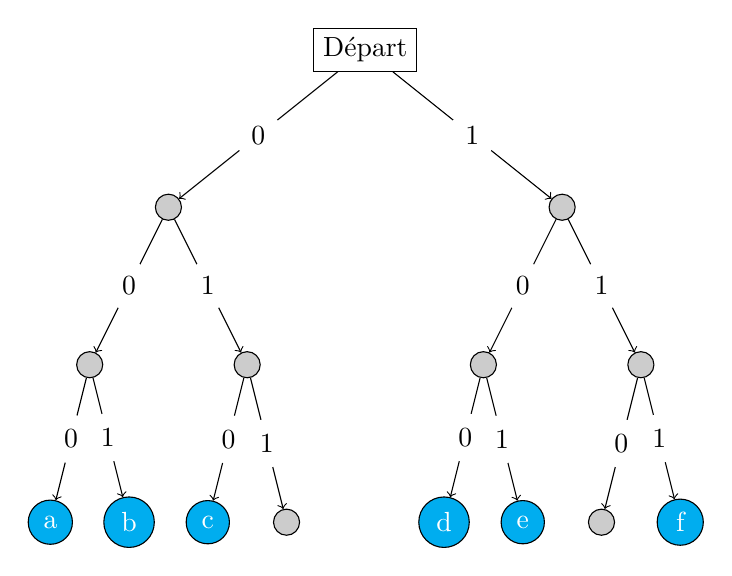
\begin{tikzpicture}[scale=1]
			\tikzstyle{etiquette}=[midway, circle ,fill=white]
			\node[draw] (D) at (0,0){Départ};	
			\node[draw, circle, fill=black!20] (1) at (2.5,-2){};
			\node[draw, circle, fill=black!20] (0) at (-2.5,-2){};
			\node[draw, circle, fill=black!20] (11) at (3.5,-4){};
			\node[draw, circle, fill=black!20] (10) at (1.5,-4){};
			\node[draw, circle, fill=black!20] (01) at (-1.5,-4){};
			\node[draw, circle, fill=black!20] (00) at (-3.5,-4){};
			\node[draw, circle, fill=cyan, text=white] (111) at (4,-6){f};
			\node[draw, circle, fill=black!20] (110) at (3,-6){};
			\node[draw, circle, fill=cyan, text=white] (101) at (2,-6){e};
			\node[draw, circle, fill=cyan, text=white] (100) at (1,-6){d};
			\node[draw, circle, fill=black!20] (011) at (-1,-6){};
			\node[draw, circle, fill=cyan, text=white] (010) at (-2,-6){c};
			\node[draw, circle, fill=cyan, text=white] (001) at (-3,-6){b};
			\node[draw, circle, fill=cyan, text=white] (000) at (-4,-6){a};

			\draw[->] (D) -- (0)node[etiquette]{0};
			\draw[->] (D) -- (1)node[etiquette]{1};
			\draw[->] (0) -- (00)node[etiquette]{0};
			\draw[->] (0) -- (01)node[etiquette]{1};
			\draw[->] (1) -- (10)node[etiquette]{0};
			\draw[->] (1) -- (11)node[etiquette]{1};
			\draw[->] (00) -- (000)node[etiquette]{0};
			\draw[->] (00) -- (001)node[etiquette]{1};
			\draw[->] (01) -- (010)node[etiquette]{0};
			\draw[->] (01) -- (011)node[etiquette]{1};
			\draw[->] (10) -- (100)node[etiquette]{0};
			\draw[->] (10) -- (101)node[etiquette]{1};
			\draw[->] (11) -- (110)node[etiquette]{0};
			\draw[->] (11) -- (111)node[etiquette]{1};
		\end{tikzpicture}\\
	\end{center}
	\begin{tabular}{r|l}
		Symbole de source & Code de Shannon-Fano\\
		\hline
		a & 000\\
		\hline
		b & 001\\
		\hline
		c& 010\\
		\hline
		c& 011\\
		\hline
		d& 100\\
		\hline
		e& 101\\
		\hline
		f&111
	\end{tabular}\\
	La longueur moyenne de ce code est $L(\Gamma_{SF}) = \frac{1}{6}\cdot(3\cdot6) = 3$, la même que celle de D.\\
	Vu que nous travaillons avec un code binaire, la seconde inégalité de l'entropie devient $H(S)+1 \geq L(\Gamma_{SF}) \geq H(S)$\\
	Nous connaissons $H(S) \simeq 2.584$, et $L(\Gamma_{SF}) = 3\\
	\to 1+2.584 = 3.584 \geq 3\geq 2.584$. La seconde inégalité de l'entropie est donc respectée.
		\item Le code $D_1$ est instantané car aucun mot n'est un préfixe d'un autre.\\
	Sa longueur moyenne est de $\frac{1}{6}(4\cdot 3 + 2\cdot 2) = \frac{16}{6} = 2,\overline{6}$. Cette longueur est plus courte que celle du code de Shannon-Fano (bien que toujours plus grande que $H(S)$). En effet, si le code de Shannon-Fano est garanti efficace, il n'est pas garanti être le meilleur ; ce code $D_1$ en est la preuve.
	\item La longueur des mots de code de Shannon se calcule comme avant ($\lceil\log_2\left(\frac{1}{p_i}\right)\rceil$)
	\begin{tabular}{r|c|c|c|c|c|c}
	Symbole de Source  & a & b & c & d & e & f\\
	\hline
	Probabilité & 0.3 & 0.2 & 0.01 & 0.08 & 0.01 & 0.4 \\
	\hline
	longueur approximative & 1.73 & 2.32 & 6.64 & 3.64& 6.64 &1.32\\
	\hline
	\textcolor{red}{longueur arrondie} & \textcolor{red}{2} & \textcolor{red}{3} & \textcolor{red}{7} & \textcolor{red}{4} & \textcolor{red}{7} & \textcolor{red}{2}
	\end{tabular}\\
	Ce qui nous donne une longueur moyenne de $L(\Gamma_{SF}) =$\fbox{2.46}\\
	La longueur moyenne de D (appliquée à $S'$) est de \\
	$2\cdot0.3 + 3\cdot 0.2 + 3\cdot0.01 + 2\cdot 0.08 + 4\cdot0.01 + 4\cdot0.4 =$ \fbox{3.03}\\
	La longueur moyenne du code $D_1$ est de \\
	$2\cdot0.3+3\cdot0.2+3\cdot0.01+2\cdot0.08+3\cdot0.01+3\cdot0.4 =$ \fbox{2.62}\\
	 L'entropie de $S'$ est de \\
	 $H(S') = -0.3\log_2(0.3) -0.2\log_2(0.2)-0.01\log_2(0.01)-0.08\log_2(0.08)-0.01\log_2(0.01)-0.4\log_2(0.4) \simeq$ \fbox{1.938}\\
	 La seconde inégalité de l'entropie est $H(S') \leq L(\Gamma_{SF}) \leq H(S')+1$ (car nous sommes en présence d'un code binaire). Nous devons donc vérifier l'inégalité suivante :\\
	$1.938 \leq 2.46  \leq 2.938 = 1.938+1$. Cette inégalité est diablement juste, nous pouvons donc affirmer que la seconde inégalité de l'entropie est respectée pour ce code.	 
\end{enumerate}~
\\
\\
\\
\\
\\
\\
\\
\\
\\
Pensez au pauvre étudiant que je suis ! Je fais un effort en faisant de magnifiques (quoi que chronophages) arbres, alors pourquoi ne pas me récompenser ? :D

\end{document}